\documentclass[a4paper,12pt]{article}

% Se vuoi che il pdf sia in formato mobile, decommenta la linea qui sotto e commenta la prima linea del codice
%\documentclass[1pt]{article}
\usepackage{enumitem}
\usepackage[paper size={90mm, 160mm},left=2mm,right=2mm,top=2mm,bottom=2mm,nohead]{geometry}
\usepackage{microtype}
\setlist[itemize]{leftmargin=*}


\usepackage{float}
\usepackage{url}
\usepackage{xcolor}
\usepackage{pdfpages}
\usepackage{graphicx}


%Comando per creare nuove definizioni stile blocco
\newcommand{\definition}[2]{
	\begin{table}[H]
	\centering
		\begin{tabular}{|p{0.9\linewidth}}
		\textbf{#1}\\ %Titolo della definzione
		#2\\%Testo della definizione
		\end{tabular}
	\end{table}
	\noindent
}

\newcommand{\df}[2]{\definition{#1}{#2}}

%%%%%%%%%%%%%%%%%%%%%%%%%%%%%%%%%%%%%%%%%%%%%%%%%%%%%%%%%%%%%%%%%%%%%
%      INSBOX --- macros for inserting pictures into paragraphs     %
%       Micha\l{} Gulczy\'nski, Szczecin, Jan 1996 / Feb 1998       %
%                     mgulcz@we.tuniv.szczecin.pl                   %
%%%%%%%%%%%%%%%%%%%%%%%%%%%%%%%%%%%%%%%%%%%%%%%%%%%%%%%%%%%%%%%%%%%%%
%
%  version 2.2
%
%  available macros:
%    * \InsertBoxC{anybox}
%        insert a centered box (use int _inside_ a paragraph)
%    * \InsertBoxL{after_line}{anybox}[correction]
%    * \InsertBoxR{after_line}{anybox}[correction]
%        insert a box in the left/right after specified number of lines;
%        correction specified in square brackets is optional;
%        both macros should be called _before_ a paragraph
%    * \MoveBelowBox
%        start a new paragraph just below the current frame
%
%  see the demo.tex file for more information
%

\catcode`\@ = 11
%
%  Margin between the text and the box:
\newdimen\@InsertBoxMargin
\@InsertBoxMargin = 2mm
%
%  definition of \ParShape, an inproved version of plain \parshape
%
\newcount\@numlines    % sum: m_1+...+m_n
\newcount\@linesleft   % counter used when reading lines of \ParShape
\def\ParShape{%
    \@numlines = 0
    \def\@parshapedata{ }% here we'll collect data for plain \parshape
    \afterassignment\@beginParShape
    \@linesleft
}%
\def\@beginParShape{%
    \ifnum \@linesleft = 0
      \let\@whatnext = \@endParShape
    \else
      \let\@whatnext = \@readnextline
    \fi
    \@whatnext
}%
\def\@endParShape{%
    \global\parshape = \@numlines \@parshapedata
}%
\def\@readnextline#1 #2 #3 {% #1 #2 #3 are: m_i, leftskip_i, rightskip_i
    \ifnum #1 > 0
      \bgroup  % I want to keep changes of \dimen0 and \count0 local
        \dimen0 = \hsize
        \advance \dimen0 by -#2  % \parshape requires left skip and
        \advance \dimen0 by -#3  % _length_of_line_ (not right skip!)
        \count0 = 0
        \loop
          \global\edef\@parshapedata{%
            \@parshapedata    % add to \@parshapedata:
            #2                % left skip
            \space            % a space
            \the\dimen0       % length of line
            \space            % another space
          }%
          \advance \count0 by 1
          \ifnum \count0 < #1
        \repeat
      \egroup
      \advance \@numlines by #1
    \fi
    \advance \@linesleft by -1
    \@beginParShape
}%
%
%  \InsertBoxC, \InsertBoxL, \InsertBoxR
%
\newbox\@boxcontent     % box containing the picture to be inserted
\newcount\@numnormal    % number of leading lines to typeset normally
\newdimen\@framewidth   % width of the frame
\newdimen\@wherebottom  % position of frame's bottom
\newif\if@byframe       % true if we are just beside the frame
\@byframefalse
%
%
\def\InsertBoxC#1{%
  \leavevmode
  \vadjust{
    \vskip \@InsertBoxMargin
    \hbox to \hsize{\hss#1\hss}
    \vskip \@InsertBoxMargin
  }%
}%
\def\InsertBoxL#1#2{%
  \@numnormal = #1
  \setbox\@boxcontent = \hbox{#2}%
  \let\@side = 0
  \futurelet \@optionalparameter \@InsertBox
}
\def\InsertBoxR#1#2{%
  \@numnormal = #1
  \setbox\@boxcontent = \hbox{#2}%
  \let\@side = 1
  \futurelet \@optionalparameter \@InsertBox
}%
\def\@InsertBox{%
  \ifx \@optionalparameter [
    \let\@whatnext = \@@InsertBoxCorrection
  \else
    \let\@whatnext = \@@InsertBoxNoCorrection
  \fi
  \@whatnext
}%
\def\@@InsertBoxCorrection[#1]{%
  \ifx \@side 0
    \@@InsertBox{#1}{0}{{\the\@framewidth} 0cm}%
  \else
    \@@InsertBox{#1}{1}{0cm {\the\@framewidth}}%
  \fi
}%
\def\@@InsertBoxNoCorrection{%
  \@@InsertBoxCorrection[0]%
}%
\def\@@InsertBox#1#2#3{%
  \MoveBelowBox
  \@byframetrue
  % \@wherebottom = \pagetotal + (\@numnormal * \baselineskip) +
  %                 (height of \@boxcontent) + (2 * \@InsertBoxMargin)
  \@wherebottom = \baselineskip
  \multiply \@wherebottom by \@numnormal
  \advance \@wherebottom by 2\@InsertBoxMargin
  \advance \@wherebottom by \ht\@boxcontent
  \advance \@wherebottom by \pagetotal
  % I have no idea why, but \InsertBox called at the top of a page
  % calculates space for the box one line too big
  \ifdim \pagetotal = 0cm
    \advance \@wherebottom by -\baselineskip  % ^ reduction
  \fi
  % add the correction
  \advance \@wherebottom by #1\baselineskip
  % \@framewidth = (width of \@boxcontent} + \@InsertboxMargin
  \@framewidth = \wd\@boxcontent
  \advance \@framewidth by \@InsertBoxMargin
  %
  \bgroup  % to keep changes of \dimen0 local
    % check if the box fits in the page
    \ifdim \pagetotal = 0cm
      \dimen0 = \vsize
    \else
      \dimen0 = \pagegoal
    \fi
    \ifdim \@wherebottom > \dimen0
      % print a warning message ...
      \immediate\write16{+--------------------------------------------------------------+}%
      \immediate\write16{| The box will not fit in the page. Please, re-edit your text. |}%
      \immediate\write16{+--------------------------------------------------------------+}%
      % ... and mark this place in document with a black box
      \vrule width \overfullrule
    \fi
  \egroup
  \prevgraf = 0
  % insert the box in the left (if #2 = 0) or in the right (if #2 = 1)
  \vbox to 0cm{%
    \dimen0 = \baselineskip
    \multiply \dimen0 by \@numnormal
    \advance \dimen0 by -\baselineskip
    \setbox0 = \hbox{y}%
    \vskip \dp0
    \vskip \dimen0
    \vskip \@InsertBoxMargin
    \ifnum #2 = 1
      \vtop{\noindent \hbox to \hsize{\hss \box\@boxcontent}}%
    \else
      \vtop{\noindent \box\@boxcontent}%
    \fi
    \vss
  }%
  % I have no idea why, but this is really necessary
  \vglue -\parskip
  \vskip -\baselineskip
  % each following paragraph needs to be formatted properly
  \everypar = {%
    % are we already below the bottom of the box?
    \ifdim \pagetotal < \@wherebottom
      % no...
      \bgroup  % to keep some changes local
        % let's calculate parameters for \ParShape
        \dimen0 = \@wherebottom
        \advance \dimen0 by -\pagetotal
        \divide \dimen0 by \baselineskip
        \count1 = \dimen0
        \advance \count1 by 1
        \advance \count1 by -\@numnormal
        \ifnum #2 = 1
          \ParShape = 3
                      {\the\@numnormal}   0cm   0cm
                      {\the\count1}       0cm   {\the\@framewidth}
                      1                   0cm   0cm
        \else
          \ParShape = 3
                      {\the\@numnormal}   0cm                  0cm
                      {\the\count1}       {\the\@framewidth}   0cm
                      1                   0cm                  0cm
        \fi
      \egroup
    \else
      % yes!
      \@restore@    % it's time to end everything
    \fi
  }%
  % this definition isn't very necessary --- just in case the paragraph
  % following \InsertBoxL or \InsertBoxR has fewer lines that the
  % first argument of the macro
  \def\par{%
      \endgraf
      \global\advance \@numnormal by -\prevgraf
      \ifnum \@numnormal < 0
        \global\@numnormal = 0
      \fi
      \prevgraf = 0
  }%
}%
%
%  call this macro to move the current position just below the
%  current frame
%
\def\MoveBelowBox{%
  \par
  \if@byframe
    \global\advance \@wherebottom by -\pagetotal
    \ifdim \@wherebottom > 0cm
      \vskip \@wherebottom
    \fi
    \@restore@
  \fi
}%
%
%  normal settings are as follows:
%
\def\@restore@{%
    \global\@wherebottom = 0cm
    \global\@byframefalse
    \global\everypar = {}%
    \global\let \par = \endgraf
    \global\parshape = 1 0cm \hsize
}%
%
%  someone told me that in LaTeX there is no \pageno counter;
%  the counterpart is \c@page
%
\ifx \documentclass \@Dont@Know@What@It@Is@
\else
  \let \pageno = \c@page
\fi


\catcode`\@ = 12

\newcommand{\lessonDate}[1]{\InsertBoxR{0}{\tiny{#1}}}

\newcommand{\E}{\`E\space}

\usepackage{listings}
\lstset{language=C++,
                keywordstyle=\color{blue},
                stringstyle=\color{red},
                commentstyle=\color{green},
                morecomment=[l][\color{magenta}]{\#}
}



\sloppy
\begin{document}

\begin{titlepage}
\begin{center}
	\Large{\textbf{Appunti di Sviluppo Software in Gruppi di Lavoro Complessi}}
\vfill
\normalsize{Caccaro Sebastiano}\\
\normalsize{A.A.2019/2020}
\end{center}
\end{titlepage}

\tableofcontents

\clearpage


%Lezione di Giovedi 4 Ottobre 2019
\lessonDate{4 Ottobre 2019}
\section{Modelli Organizzativi}
Lo sviluppo software presenta dei problemi intrinseci:
\begin{itemize}
\item \textbf{Non linearità del software}: Un errore molto piccolo può avere conseguenze catastrofiche
\item Obiettivi poco chiari e mutabili
\end{itemize}
Questi problemi esistono tutt'oggi e sono difficilmente mitigabili. Esistono invece delle criticità che possono essere risolte.

\definition{Legge di Brooks}{Aggiungere personale ad un progetto in ritardo lo farà solo ritardare.}

Nello sviluppo software, non tutto è facilmente parallelizzabile. Non posso far nascere un bambino da 9 donne in un mese. Va da se che l'\textbf{effort} non corrisponde al \textbf{progress}. \`E molto facile stimare quanto si è lavorato, è meno facile misurare di quanto si è progredito, e questo può causare ulteriori ritardi. La soluzione non è aggiungere personale.

Un progetto deve mantenere sempre la sua \textbf{integrità concettuale}.\\
Per far ciò Brooks propone vari modelli.

\subsection{Modelli a Cattedrale e sala Operatoria}
\begin{itemize}
\item \textbf{Cattedrale}: Tenere rigorosamente separata progettazione e implementazione. L'implementatore deve quindi curarsi solamente di seguire quanto progettato. Si mantiene così la visione originale del progetto. Questo modello ha però il difetto di essere molto poco flessibile, e difetti nel progetto comportano problematiche enormi.
\item \textbf{Sala operatoria:} Solamente il chirurgo (superbravo) si occupa di fare le cose importanti, gli altri nella sala fanno praticamente solo da assistente. Il vero lavoro viene svolto solamente dal chirurgo (una sola persona).
\end{itemize}
Questi modelli fanno però due grosse supposizioni:
\begin{itemize}
\item Che sia possibile accentare lo sforzo creativo in un'unica persona.
\item Che sia possibile separare completamente progettazione e implementazione.
\end{itemize}
La maggior parte delle volte, tuttavia, queste supposizioni non si rivelano corrette.

\subsubsection{Critiche}
Eric Raymond contrappone il modello a \textbf{bazaar} (usato per lo sviluppo di Linux) contro la cattedrale di Brooks, osservando che il modello open source di Linux produca software di qualità, pur non usando i modelli proposti da brooks.
\lessonDate{8 Ottobre 2019}

\subsection{Modello a Bazaar}
Usato in Linux, si identifica esplicitamente come l'antitesi del modello a cattedrale. Raymond condivide l'analisi di Brooks, ma arriva alla conclusione che ci possano essere altri modelli in certe situazioni.
\definition{Baazar}{Mercato autogestito, dove chiunque può mettere una bancarella dove vuole, quando vuole}

\begin{figure}[H]
	\centering
	 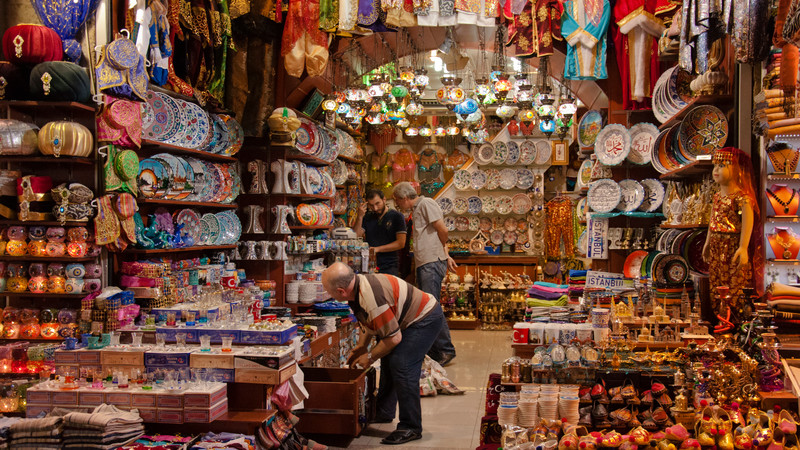
\includegraphics[width=0.6\linewidth]{Immagini/bazaar.jpg}
	 \caption{Un bazaar}
\end{figure}

Nel modello a Baazar, ognuno fa i propri interessi e sviluppa ciò che gli interessa sviluppare. Non c'è quindi un obiettivo comune, ma nel perseguire i propri interessi chi sviluppa nel modello a Baazar contribuisce a tenere viva la codebase. Questo processo non segue un modello prefissato, e quindi produce una sorta di organismo in continua evoluzione, il quale scopo quindi non diventa obsoleto.
Ma cosa permette a progetti come questi, che non adottano i modelli di Brooks, di non fallire?
\begin{itemize}
 \item Le persone non lavorano perchè costrette a farlo per un'azienda. Chi contribuisce lo fa per interessi personali, ed è quindi interessato e motivato ("personal itch")
 \item Gli utenti sono considerati co-sviluppatori, ciò aiuta a individuare e risolvere bug più velocemente
 \item Rilasciare presto e frequentemente, in modo tale da avere sempre feedback
\end{itemize}

\definition{Legge di Linux}{Data una base di beta-tester e co-sviluppatori abbastanza amplia, quasi ogni problema può essere scoperto e risolto velocemente da qualcuno.}

Per Brooks un numero elevato di utenti porta inevitabilmente ad avere più bug, in quanto ogni utente può vedere problemi diversi. Raymond invece considera gli utenti come collaboratori, che possono aiutare lo sviluppatore.\\
Anche questo modello, in teoria fantastico, in pratica è abbastanza idealistico.

\subsection{Modello a Kibbutz}
Per poter supportare delle applicazioni, un sistema deve fornire dei servizi adeguati, come kernel, driver, librerie di sistema ecc.\\
Linux è solamente un kernel, non ci si possono far girare applicazioni. Nasce quindi li concetto di \textbf{distribuzione}, ovvero un sistema completo immediatamente utilizzabile. Un programma viene quindi distribuito sotto forma di pacchetto, che è progettato per lavorare con una distribuzione (esempio pacchetto .deb).

\definition{Kibbutz}{Fattoria, villaggio, impresa collettiva nata in Israele, con scopo di popolare il nuovo stato}

\begin{figure}[H]
	\centering
	 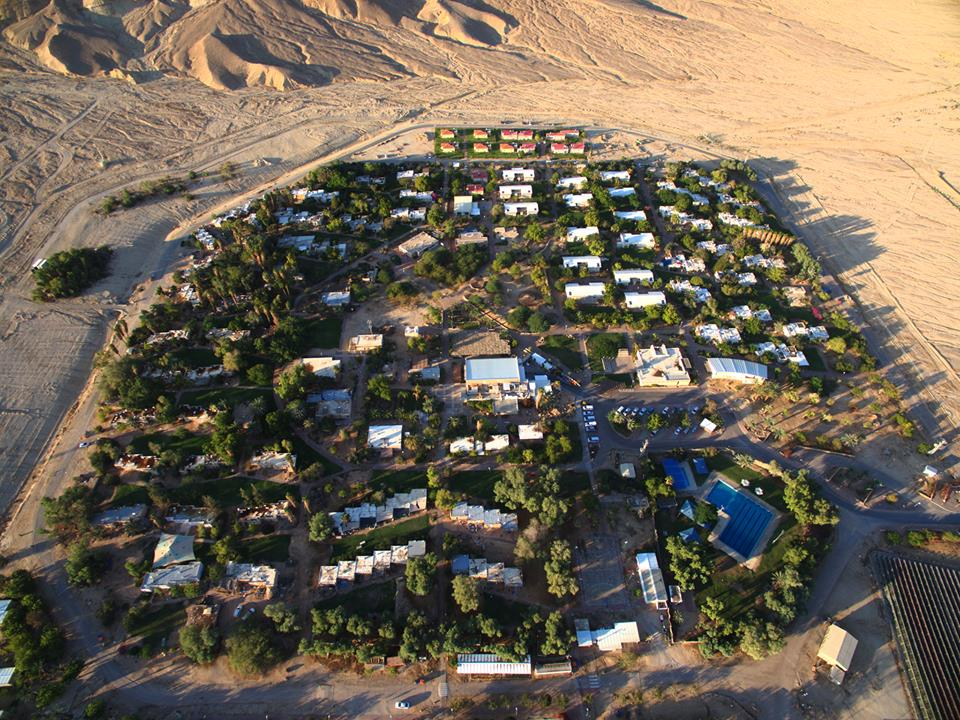
\includegraphics[width=0.6\linewidth]{Immagini/kibbutz.jpg}
	 \caption{Un kibbutz}
\end{figure}

Non parliamo quindi più di un bazaar, dove ognuno fa quello che vuole. Ma di un'organizzazione strutturata e organizzata, con uno scopo comune. Sono presenti delle \textbf{policy} prestabilite, che hanno dei corrispettivi tool che assicurano il rispetto di tali policy. Queste policy hanno l'effetto di abbassare drasticamente l'effort comunicativo fra i vari contributori al progetto. Praticamente molti progetti open-source sono organizzati a kibbutz, perchè il modello a Baazar non è una strada viabile. 
\\Questa è la filosofia adottata da Debian.

\subsubsection{Esempio di Debian}
Fin dall'inizio, Debian è openSource (ad oggi circa 1900 sviluppatori, che devono superare degli esami). Supporta più di 10 architetture e tre kernel diversi (una distribuzione non è per forza linux).\\
In Debian, ogni pacchetto contiene alcune informazioni come:
\begin{itemize}
 \item Nome
 \item Architetture supportate
 \item \textbf{Dipedenze}: tutti i pacchetti che servono al corretto funzionamento del mio pacchetto. Il solo codice sorgente del mio pacchetto è inutile senza queste informazioni
\end{itemize}

Nel pacchetto sono contenuti anche i propri file di configurazione. Questi file sono specificati nei pacchetti, quindi un upgrade non va a intaccare la configurazione. In caso ci siano problemi, chiedo all'utente di fare il merge.

\lessonDate{10 Ottobre}
\section{Metodologie Agili}
Negli anni 90 si pensa che il modo per aumentare la qualità di processi debba dipendere da una gran enfasi sulla produzione di documentazione, UML ecc. Nascono quindi dei nuovi modelli organizzativi che reagiscono a queste cose pallose, come:
\begin{itemize}
\item eXtreme Programming
\item Scrum
\end{itemize}
Il manifesto della \textbf{Programmazione Agile} viene pubblicato nel 2001, ed esprime i seguenti concetti:
\begin{enumerate}
\item Individui e interazioni \textgreater\space Processi e strumenti
\item Software funzionante \textgreater\space Documentazione esaustiva
\item Collaborazione cliente \textgreater\space Negoziazione contratti
\item Rispondere al cambiamento \textgreater\space Seguire un piano
\end{enumerate}
Tutti questi punti sono un però \textbf{molto generici e idealistici}, e sono sì belli, ma poco applicabili. Il più concreto di questi è forse il punto 4, perchè riconosce il fatto che è molto facile sbagliare la pianificazione. \E meglio quindi salvare risorse per potersi adattare a nuove situazioni.

\end{document}
